\documentclass[]{report}
\usepackage{url}
\usepackage{graphicx}
\usepackage{amsmath,amssymb}
\usepackage[numbers]{natbib}
\usepackage{titlesec}
\usepackage{appendix}
\usepackage{pdfpages}
\usepackage{verbatim}

% Title Page
\title{Evaluation Report}
\author{Liam Brand}
\date{}


\begin{document}
\maketitle

\section{The System Produced}
The overall project aim was to develop a prototype system that involves several sensors monitoring an environment, and then using the data acquired from this for analytics and visualization through an appropriate medium. This section aims to explore the implemented features with regards to how well they were implemented according to various criteria.

	\subsection{Fitness for Purpose}
	Subsystems were successfully implemented to meet the overall project goal outlined earlier. Two sensors were developed that posted data to a database, and a front end containing appropriate functionality for data visualization and analysis was created as well. The visualization and analysis subsystems were also made capable of communication with both devices, allowing the system to communicate with multiple environmental sensors. The physical demo was proof of the product's functionality.
	
	As well, these elements have been implemented to be near real-time, as stored and processed data needs to be up to date for the system to be accurate. Analysing an hour old reading for example might not provide useful information as it's uncertain whether or not this reading represent the environment's current state. The sensors post their readings to the database every 15 seconds, allowing for the database to receive sensory data at a relatively quick pace. As well, XML http requests have been configured to fire every few seconds for relevant data visualization and data analysis methods, ensuring what is displayed or analysed is the most up to date information available and provides the most value to the user.
	
	Adherence to industry standards was also achieved where possible. For example, the model features an ability to inform users of problematic temperature differences between sensors. When discussing temperature differences between rooms, IBACOS - a strategic partner of the US Department of Energy - notes that "Room-to-room temperature differences or floor-to-floor temperature differences should be no greater than 4°F in the heating season"\cite{burdick2011advanced}. The model therefore used this as a guide for its temperature difference threshold, but unknowns such as the temperature location, potential for sensory noise and use of only one sensor rather than one for each room, so the threshold was increased to four degrees celsius to accommodate for these aspects.
	
	%During their investigation of a heating system, IBACOS notes\cite{thermalcomfortibacos} that the ACCA (Air Conditioning Contractors of America) has a standard of no more than four degrees fahrenheit (almost two and a half celsius) difference between rooms. This standard was used for their experiments in determining how viable their heating system was, and indeed is recognized by the wider industry. @techreport{thermalcomfortibacos,
	%title={Thermal Comfort Performance},
	%institution={Integrated Building and Construction Solutions},
	%note={Available at: \url{https://cdn.ymaws.com/www.nibs.org/resource/resmgr/BEST/BEST1_045.pdf} (Accessed 01/05/19)}
	%}
	
	\subsection{Robustness}
	AWS Lambda is used, which features functionality to allow scaling\cite{awslambdadocs} allowing the database to cope with additional device implementations. The devices themselves have features to cope with failures. It features two temperatures sensors with the second one being used if the first one fails, features in code to prevent erroneous measurements. As well, the devices will automatically attempt to reestablish internet connection upon being disconnected, and they also feature a 32GB Micro-SD card as temporary storage for readings data should connection be lost. Web elements such as the model's code contains try/catch statements to handle exceptions such as empty readings from the database as well, and will print appropriate messages to the console to assist in troubleshooting should these issues occur.
	
	\subsection{Look and Feel}
	Petrie and Fraser\cite{petrie2004tension} describe many different issues that significantly impede users' ability to properly make use of a website. The primary offenders here are complex pages, unclear navigation and poor colour contrast. The website's pages are very simple, with large block elements for listed devices and clear headings denoting sections such as the intelligent model's device comparison results. Navigation is achieved via the use of a simple navbar, something seen very often in websites and shouldn't be unfamiliar to users that have used other websites before. As well, the website's colour scheme is mainly dark blue and white, offering a clear contrast between the background and elements such as text. These elements allow the system's interactive element to be intuitive, familiar, easy to use and visually pleasing.
	
	\subsection{Consistency}
	Subsystems have been developed with other subsystems in mind. For example, the website front end was properly formatted to make space for the data visualization and data analytics. These elements have clear areas of the web page reserved for them that allows them to blend into the rest of the website, and they were included in the media queries to allow the website to scale to different screen sizes. The database features endpoints allowing the developed sensors to post data to the database, and endpoints were also created to provide the visualization and analysis subsystems with the sensory data that they needed to perform their functions. These things allowed the subsystems to work together without anything feeling out of place or not accommodated for.
	
	\subsection{Technical Evaluation}
	The technology used was appropriate to the subsystem it was employed for. The devices used sensors that gathered relevant data, the database allowed the creation of needed endpoints and included the inbuilt scaling technology, and the front end subsystem's usage of HTML, CSS and PHP allowed for a pleasant looking and well working website. The use of JavaScript in particular for the visualization and model subsystems allowed for the creation of automated HTTP requests that ran every few seconds. This allowed for the regular retrieval of relevant data from the database which helped these systems be accurate as they always use the latest data available in the database, and as such the latest data from the sensor.
	
	Regarding code quality, code featured appropriate comments, indentations and method/variable names to maximize code readability. Proper functional decomposition was done where appropriate as well. For example in the model, part of determining an ideal temperature was to look at temperature readings from the same time for previous days. For this, timestamps needed to be created so readings made around these times could be searched for and retrieved. Creation of these timestamps was initially done in the \textit{checkTemperature} method, but it was later turned into a \textit{getPreviousTimestamps} helper function to maximize readability and group together relevant code.
	
	\subsection{Non-Functional Requirements}
	Primary non-functional requirements concerned the webapp's usability and the appropriate rate at which data was retrieved from the sensors and processed. These aspects have already been covered in previous sections. There is also a requirement for the development of an economic model to help cost the intelligent model, which can be found in the appendices.
	
	%\subsection{Financial Breakdown}
	%As part of the model's development, the system's implementation needs to be financially evaluated to determine the cost of its deployment on an industrial level. The Terms of Reference outlines the project's main finances, but here will be a more in depth exploration of the financial aspects behind the model specifically.
	%If the model was to continue being used in its current form
	%\cite{awsp2instancedocs}

\section{Project Management, Process and Personal Achievement}
	\subsection{Terms of Reference}
	The description of subsystem requirements helped aid development by providing an understanding of the scope, complexity and methods/technologies that will be used for their implementation. For example, the model's specification helped bring up some early questions regarding the model's possible behavior (e.g. what to do if it's too hot) and this allowed the developer to know what needed to be understood before development could begin. Discussion of the project's testing could have used more depth however, and things like unit testing (and perhaps the respective testing frameworks for the different technologies being used) could have been mentioned.
	
	\subsection{Requirements and Design Documentation}
	Wireframes for the website's front end were created, these helped in understanding how the final website would look which helped front end development, and also allowed the data visualization and model subsystems to understand how their respective information should be output so that it can fit into the created website (e.g. how do we tell the user it's too hot in a way that displays well on the designed page?).
	
	Pseudo code might have been useful for the elements such as the model to give the group a clear understanding of the subsystem's technical implementation.
	
	\subsection{Time Management}
	Most time objectives were met, with development concluding in April as shown by the meeting minutes' satisfaction of a live end to end product by March. Development primarily finished mid April however rather than the start of April, so a more thorough understanding of task complexity and needed development time is required. The plan was however, for the most part, stuck to well.
	
	\subsection{Configuration Management and Integration Strategies}
	Both configuration and integration was primarily managed through the use of version control. A global repository was created with each group member added as a collaborator, and changes were committed and pushed to their own branches where appropriate. These branches were reviewed to determine their compatibility with existing code and merged into the master branch after. This ensured that all written code fit together without breaking other elements, and also provided a global repository accessible by each group member for the project's source code. Integration of subsystems was also discussed during meetings, for example the meeting on the 25th of March features an end to end demo utilizing all subsystems together as an objective.
	
	\subsection{Testing Strategies}
	Use of the project during code merges on git ensured that code updates didn't break the project, and a live end to end demo was conducted prior to the demonstration to ensure all features worked. A more thorough style of integration testing with a sophisticated testing plan would have been better however, and unit tests for specific code elements would have helped ensure system stability.
	
	\subsection{Group Leadership}
	No leader was elected among the group, this had issues in determining solid internal deadlines on different pieces of functionality. Likely this is one of the reasons that the project's time plan couldn't be properly adhered to.
	
	\subsection{Quality Planning}
	Group members inspected each others developed code to look for faults overlooked during initial development. These code reviews helped prevent tunnel vision where issues are repeatedly overlooked. To increase efficiency, notes could be made from these code reviews and published in a group folder for others to see, so they can check their own code during development for similar mistakes.
	
	\subsection{Potential Additional Functionality}
	As of right now the visualization and analysis subsystems are hard coded to only retrieve data from the two created devices, moving forward this should be made more dynamic to accommodate for additional created devices to allow these subsystems to function properly as more devices are added. In addition, the data visualization could be scaled up to display data from longer periods of time (e.g. months or years). Also, the data analysis is limited in what it does with the information it learns. For example if gas or an extremely high temperature is detected in a reading this manifests through website alerts, but a fully realised product could notify the appropriate services automatically to help the user. Important notifications could also be harder to miss, sending them to the users phone as a regular mobile notification. These aspects may have been achievable with better time management.
	
	%The model could also record discrepancies and log them to a file, and potentially automatically submit timestamps and anomalous readings to the user's energy provider to help open a support ticket to resolve these issues.
	
	\subsection{Problems Encountered, Their Solutions, and Lessons Learned}
	Better time management could have been achieved from sticking to the project plan, in future more attention will be paid to these time plans to prevent falling behind too much. Also, a better idea of whether or not to have a leader will allow more discipline in sticking to self imposed deadlined, so in future it would be better to explicitly discuss whether or not the group will have a leader and if so, who it is.
	

%\subsection{Requirements Gathering}
%Requirements were gathered through the use of client questionnaires and interviews. Whilst the overall requirements of the system were already known, this allowed us to answer some questions about finer details that came up during the initial planning and distribution of work. I encountered a missed opportunity for some important information with the questionnaires however. An element of my subsystem was using weather data to help gauge whether or not the client's house temperature was comfortable, but it would have been useful to have some input on precisely how this would be done. For example, following an external temperature spike/drop does the client want the heating instantly adjusted or done slowly over a period of time to prevent it feeling uncomfortable? Do they perhaps want to be able to opt out of this small feature due to the potential inconsistency of weather forecasts and simply fine tune their house temperature themselves?

\section{Professional Issues}
The Code of Conduct was adhered to with good collaboration between teammates, as each member showed up to the group meetings and gave fair warning if other commitments would cause them to be late. Members were polite whilst still offering fair criticism. Moving forward these standards would need to be strictly adhered to, as insufficient communication between team members could cause project issues that directly affect clients causing a loss of faith in the company and as such the developed product.

\section{Legal Issues}
Data breaches against stored data were considered during the TOR. The usage of AWS helped mitigate this, with their databases featuring implemented security measured\cite{awsdatabasedocs} such as encryption and private keys required for endpoint access helping ensure the stored data is private. The repository containing the project's source code was also private with read and write privileges only given to group members, to prevent source code leaks. Terms of use such as copyright conditions were also adhered to, for example the AWS service terms\cite{awsserviceterms} were reviewed against proposed project functionality to ensure what we were using them for was acceptable by Amazon. These terms included things like ensuring the only data stored on the database was lawfully obtained by us, and these terms would need to be kept in mind once other users come into the picture should the product be deployed industrially. 

As well, the Data Protection Act\cite{dataprotectionact2018} will need to be considered should the project be deployed. In particular, the Act states that a person has the right to find out what data relating to a person is stored by an organisation. Facilities to provide customers with this data if they request it should be set up. It also states data shouldn't be kept for longer than is needed, so it should be determined how long sensory data is required for the system's ideal function and then functionality should be in place to ensure data that is no longer needed is properly disposed of. 


\section{Social Issues}


\section{Ethical Issues}

	\bibliographystyle{plainnat}
	\bibliography{papers}
	\newpage
	\begin{appendices}
		\verbatiminput{log.txt}
		
\includepdf[pages=-]{tor.pdf}
		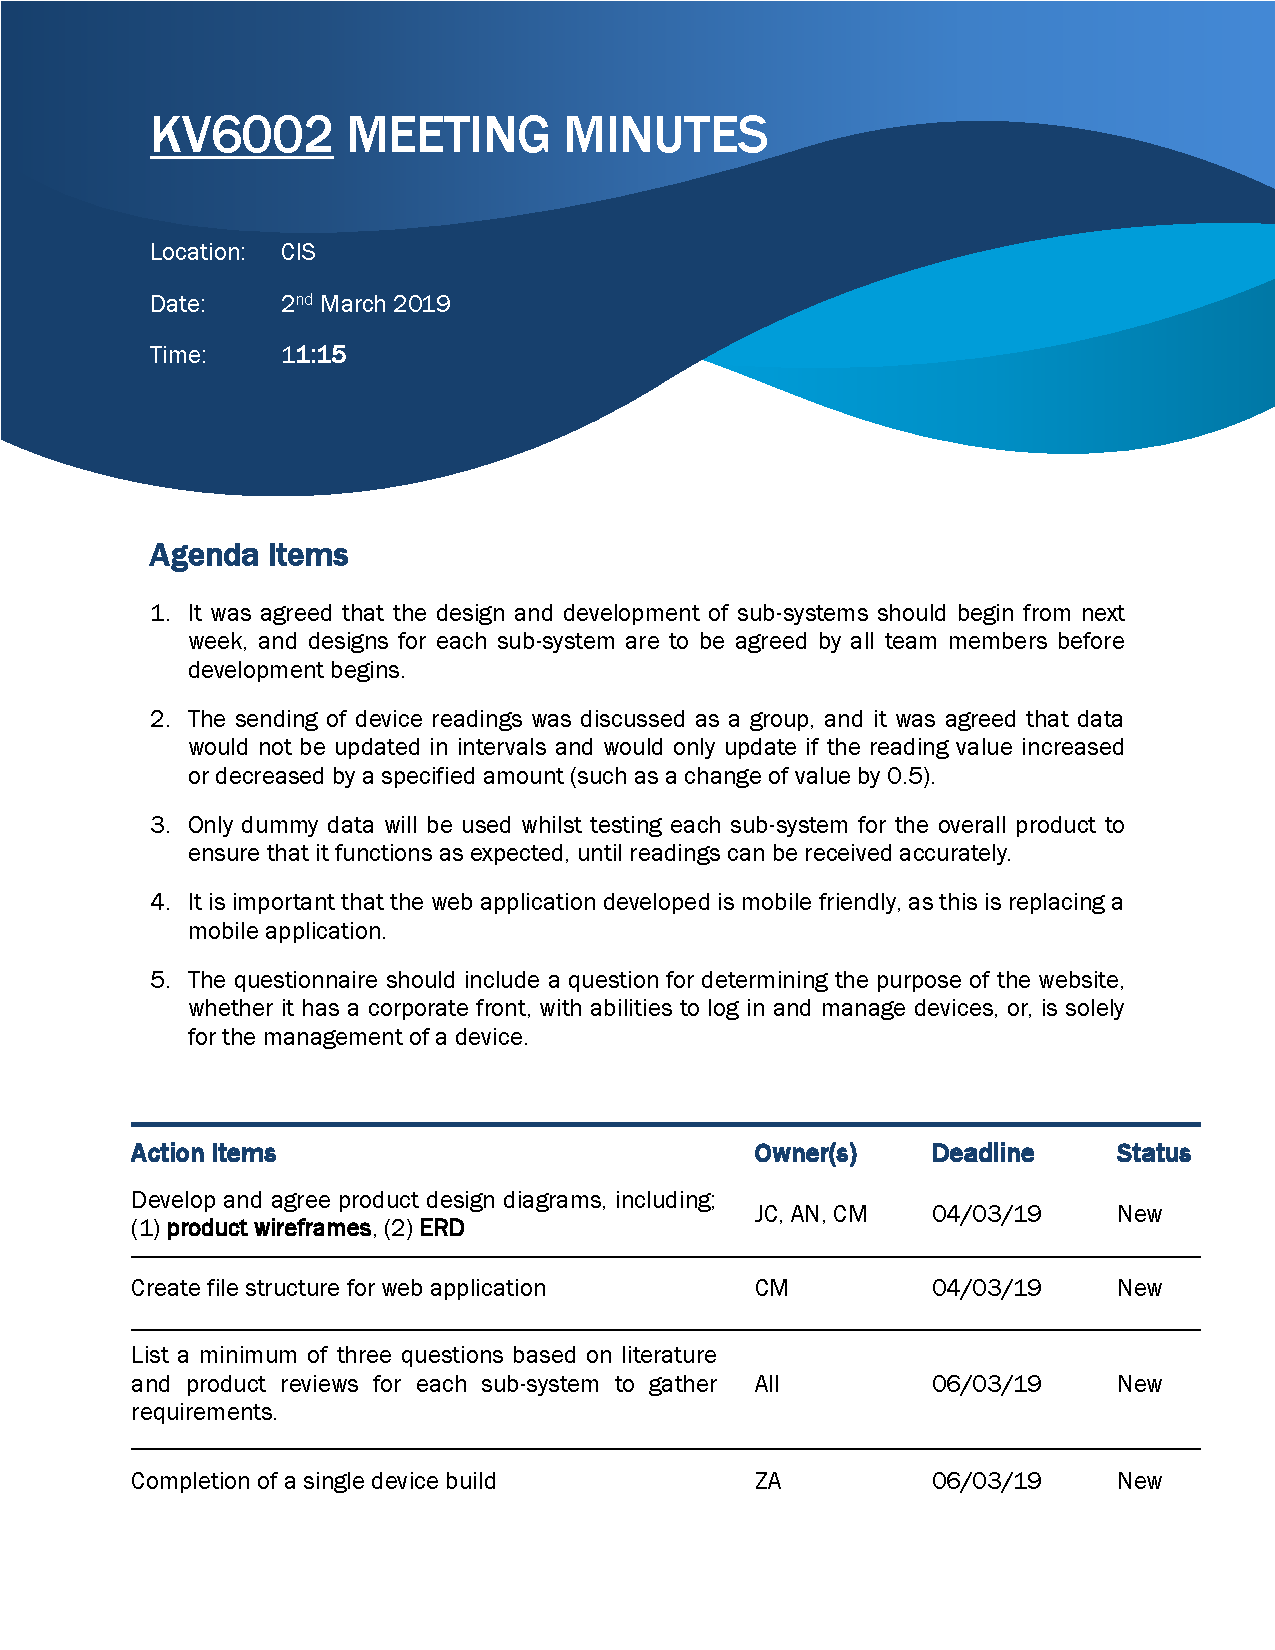
\includepdf[pages=-]{meetingminutes.pdf}
	\end{appendices}
\end{document}          
